\documentclass[11pt]{article}
\usepackage{graphicx}
\usepackage[utf8]{inputenc} 
\usepackage{epstopdf}
\usepackage[makeroom]{cancel}
\usepackage{framed}
\usepackage{cite}
\usepackage{hyperref}
\usepackage{amsmath}
\usepackage{amsfonts}

\begin{document}
\title{FYS4150: Project 1}
\author{Ingrid A V Holm}
\maketitle

\begin{abstract}
In this project we have compared numerical algorithms for the solving of differential equations. The algorithms investigated are Gaussian elimination, both a general version for tridiagonal matrices and one specific for the system under consideration, and LU-decomposition followed by inverting matrices. In light of computed errors and CPU time, LU-decomposition proved to be the least efficient.
\end{abstract}

\begin{center}
For all programs and plots used, see: \url{https://github.com/ingridavh/compphys1/tree/master/FYS4150_project1}
\end{center}


\section*{Introduction}

\begin{flushleft}

To my humble knowledge, there are virtually no problems in physics which cannot be formulated as differential equations. In quantum mechanics Schrödinger's equation describes how a quantum state evolves in time, and in electromagnetism the electrostatic field produced by a charge distribution can be calculated using Poisson's equation:

\begin{equation}
\begin{matrix}
\nabla^2 \phi = \rho & &&&&&\textit{Poisson's equation}\\
\end{matrix}
\end{equation} 

By discretizing Poisson's equation it can be solved numerically using several techniques. Gaussian elimination and LU-decomposition are amongst standard algorithms used, and they require different central processing unit (CPU) times and render different relative errors.
\end{flushleft}

\pagebreak

\section*{Methods}


\begin{flushleft}

\textbf{Poisson equation}

In three dimensions Poissons equation is:

\begin{equation}
\nabla^2 \Phi = -4 \pi \rho (\textbf{r})
\end{equation}

For a spherically symmetric potential and distribution (meaning that $\rho \neq \rho( \theta, \phi)$), this simplifies to:

\begin{equation*}
\frac{1}{r^2} \frac{d}{dr} \Big( r^2 \frac{d \Phi}{dr} \Big) = -4 \pi \rho (r)
\end{equation*}

By substituting $\Phi (r) = \frac{\phi(r)}{r}$:

\begin{equation*}
\frac{d^2 \phi}{dr^2} = -4 \pi r \rho (r)
\end{equation*}

Which is a variation of a more general form

\begin{equation}
-u''(x) = g(x)
\end{equation}

With Dirichlet boundary conditions:

\begin{equation*}
\textbf{ } x \in (0,1), \textbf{ } u(0) = u(1) = 0
\end{equation*}

\textbf{Approximation by discretization}

The discretized approximation is done by choosing $N+2$ points in the interval $(0,1)$ with equal spacing $h = \frac{1}{N+1}$. $x_i$ is then given by $x_i = x_0 + ih$, so that $x_0 = 0$ and $x_{N+1} = 1$. $u(x)$ is approximated by the functional points $v_i = v(x_i)$. The second derivative can then be approximated using the 3 point formula \cite{morken2013numerical}:

\begin{equation}
- \frac{v_{i+1} + v_{i-1} - 2 v_i}{h^2} = g_i 
\end{equation}

For $i = 1,2,...,n$, where $g_i = g(x_i)$. The mathematical error of this method is of the order of $O(h^2)$ \cite{morken2013numerical}. We wish to calculate the approximation $v(x)$ by rewriting the equation:

\begin{equation}
- v_{i-1} + 2 v_i - v_{i+1}= h^2 g_i 
\end{equation}

Setting in $i = 1,2,3...$ we start to see a pattern:

$$
- v_0 + 2 v_1 - v_2= h^2 g_1 
$$

Since $v_0 = 0$:

$$
2 v_1 - v_2= h^2 g_1 
$$

$$
- v_1 + 2 v_2 - v_3= h^2 g_2 
$$

$$
- v_2 + 2 v_3 - v_4= h^2 g_3 
$$

The discretized approximation is a matrix equation:

$$
\begin{pmatrix}
2 & -1 & 0 &...& ... & 0\\
-1 & 2 & -1 & 0 & ... & ...\\
0 & -1 & 2 & -1 & 2 & ...\\
& ... & ... & ... & ... & ...\\
0 & ... & & -1 & 2 & -1\\
0 & ... & & 0 & -1 & 2\\
\end{pmatrix}
\begin{pmatrix}
v_1\\
v_2\\
...\\
...\\
...\\
v_n\\
\end{pmatrix}
=
\begin{pmatrix}
f_1\\
f_2\\
...\\
...\\
...\\
f_n\\
\end{pmatrix}
$$

\begin{equation}
\textbf{A} \textbf{v} = \textbf{f}
\end{equation}

With $f_i = h^2 g_i$.
\end{flushleft}

\begin{flushleft}

\textbf{Specific conditions for this project}

The following source term and closed-form solution are assumed:

\begin{equation}
g(x) = 100e^{-10x}
\end{equation}

\begin{equation}
u(x) = 1 - (1-e^{-10})x - e^{-10x}
\end{equation}

A quick calculation can easily verify that these satisfy the Poisson equation (I leave this up to the sceptical reader).
\end{flushleft}


\begin{flushleft}
\textbf{Gaussian elimination}

The set of equations can be written in terms of a general tridiagonal matrix:

$$
\begin{pmatrix}
b_1 & c_1 &  & \text{\huge0}\\
a_2 & b_2 & c_2 &... \\
& ... & ... & ...\\
&   a_{n-2} & b_{n-1} & c_{n-1}\\
\text{\huge0}&  & a_n & b_n\\ 
\end{pmatrix}
\begin{pmatrix}
v_1\\
v_2\\
...\\
...\\
...\\
v_n\\
\end{pmatrix}
=
\begin{pmatrix}
f_1\\
f_2\\
...\\
...\\
...\\
f_n\\
\end{pmatrix}
$$

Which in index notation becomes:

\begin{equation}
a_i v_{i-1} + b_i v_i + c_1 v_{i+1} =f_i
\end{equation}

With $a_1= c_n = 0$. 
\end{flushleft}

\begin{flushleft}
The matrix can be transformed into a diagonal matrix by manipulating the rows, thereby solving all the equations. The metod of Gaussian elimination consists of multiplying the first row by $\frac{a_2}{b_1}$ and subtracting it from the second row. The same procedure is done for the third row, only with the second column element. This yields an upper diagonal matrix, which can be turned into a diagonal matrix by substituting the bottommost element into the row directly above, and repeating for the preceding rows.
\end{flushleft}

$$
\begin{pmatrix}
a_{11} &  ... & a_{1n}\\
... & &... \\
a_{n1} & ... & a_{nn}\\
\end{pmatrix}
\rightarrow
\begin{pmatrix}
a_{11} &...& \tilde{a_{1n}}\\
&& ... \\
\text{\huge0} & & \tilde{a_{nn}}\\
\end{pmatrix}
\rightarrow
\begin{pmatrix}
\tilde{\tilde{a_{11}}} & \text{\huge0}\\
&...\\
\text{\huge0} & & \tilde{\tilde{a_{nn}}}\\
\end{pmatrix}
$$

\begin{flushleft}

The algorithm thus consists of two steps; a decomposition and forward substitution followed by a backward substitution \cite{hjorth2011computational}:

\begin{figure}[ht]\label{Gaussian algorithm}
\begin{framed}
\begin{minipage}[b]{0.45\linewidth}
\centering
\textbf{Step 1: decomposition and forward substitution}
\begin{equation}\label{Gaussian step 1-1}
\beta_i = b_i - \frac{a_i c_{i - 1}}{\beta_{i-1}};
\end{equation}

\begin{equation}\label{Gaussian step 1-2}
\tilde{f}_i = f_i - \frac{a_i \tilde{f}_{i-1}}{\beta_{i-1}};
\end{equation}
\end{minipage}
\hspace{0.5cm}
\begin{minipage}[b]{0.45\linewidth}
\centering
\textbf{Step 2: backward substitution}
 
\begin{equation}\label{Gaussian step 2}
v_{i-1} = \frac{\tilde{f}_{i-1} - c_{i-1} v_i}{\beta_{i-1}};
\end{equation}

Where we set $\beta_0 = b_0$, $\tilde{f}_0 = f_0$ and $v_0 = v_{n+1} = 0$, $v_n = \frac{\tilde{f}_n}{\beta_n}$
\end{minipage}
\end{framed}
\caption{Gaussian elimination algorithm for tridiagonal matrix}
\end{figure}

\end{flushleft}

\begin{flushleft}
The number of \textbf{floating point operations}, or flops, is the number of additions, subtractions, multiplications and divisions performed. (\ref{Gaussian step 1-1}), (\ref{Gaussian step 1-2}) and (\ref{Gaussian step 2}) each require 3. In total we have $6$ flops for one iteration of step 1, and $3$ flops for step 2. $N-1$ iterations thus requires $6(N-1) + 3(N-1) = 9(N-1)$ flops.
\end{flushleft}


\begin{flushleft}

\textbf{Specialized algorithm}

A specialized algorithm can be found in the present case, because the coefficients are $b_i = 2$, $a_i = c_i = -1$ for all $i$. Setting this into (\ref{Gaussian step 1-1})-(\ref{Gaussian step 2}) yields:

$$
\beta_i = 2 - \frac{1}{\beta_{i-1}} 
$$

Which can be re-expressed as: 

$$
\beta_1 = 2 - \frac{1}{2} = \frac{3}{2}
$$

$$
\beta_2 = 2 - \frac{2}{3} = \frac{4}{3}
$$

$$
\beta_3 ... \rightarrow \beta_i = \frac{i+1}{i}
$$


$$
\tilde{f}_i = f_i - \frac{- \tilde{f}_{i-1}}{\frac{i}{i-1}} = f_i + \frac{i-1}{i} \tilde{f}_{i-1}
$$


$$
v_{i-1} = \frac{\tilde{f}_{i-1} + v_i}{\frac{i}{i-1}} = \frac{i-1}{i} (\tilde{f}_{i-1} + v_i)
$$

The algorithm is then:

\begin{figure}[ht]\label{Specialized algorithm}
\begin{framed}
\begin{minipage}[b]{0.45\linewidth}
\centering
\textbf{Step 1}
\begin{equation}\label{Specialized step 1-1}
\beta_i = \frac{i+1}{i};
\end{equation}

\begin{equation}\label{Specialized step 1-2}
\tilde{f}_i = f_i + \frac{i -1}{i}\tilde{f}_{i-1};
\end{equation}
\end{minipage}
\hspace{0.5cm}
\begin{minipage}[b]{0.45\linewidth}
\centering
\textbf{Step 2}

\begin{equation}\label{Specialized step 2}
v_{i-1} = \frac{i-1}{i} (\tilde{f}_{i-1} + v_i);
\end{equation}

where we set $\beta_1 = b_1 = 2$, $\tilde{f}_i = f_i$ and $v_n = \frac{\tilde{f}_n}{\beta_n}$
\end{minipage}
\end{framed}
\caption{Specialized matrix algorithm}
\end{figure}

\end{flushleft}

\begin{flushleft}
Since $\beta_i$ can be calculated beforehand, it's derivation does not contribute to the number of floating point operations. Not considering the operations between $i$'s, (\ref{Specialized step 1-1}) requires $0$ flops, (\ref{Specialized step 1-2}) requires $2$ and (\ref{Gaussian step 2}) requires 2. $N-1$ iterations require $2(N-1) + 2 (N-1) = 4(N-1)$ flops. Note that this is less than half of what is required by the regular Gaussian elimination.
\end{flushleft}



\subsection*{LU-decomposition}

\begin{flushleft}
The matrix $A$ can be decomposed into a lower- and upper diagonal matrix \cite{lindstrom2011flervariabel}

\begin{equation}
A \textbf{x} = LU \textbf{x} =  \textbf{u}
\end{equation}

Once $L$ and $U$ are found (we use the linear algebra library Armadillo to calculate these),  the unknown $\textbf{x}$ is calculated in two steps. The following contractions are used:

\begin{equation*}
L \textbf{x} = \textbf{u} \textbf{ ; } U \textbf{x} = \textbf{y}
\end{equation*}

\begin{figure}[ht]\label{LU algorithm}
\begin{framed}
\begin{minipage}[b]{0.45\linewidth}
\centering
\textbf{Step 1}
\begin{equation}
\textbf{y} = L^{-1} \textbf{u}
\end{equation}
\end{minipage}
\hspace{0.5cm}
\begin{minipage}[b]{0.45\linewidth}
\centering
\textbf{Step 2}
\begin{equation}
\textbf{x} = U^{-1} \textbf{y}
\end{equation}
\end{minipage}
\end{framed}
\caption{LU-decomposition algorithm}
\end{figure}


\end{flushleft}

\pagebreak

\section*{Results}

\subsection*{Gaussian elimination}

\begin{flushleft}
A comparison of the Gaussian elimination method for several values of N shows that the approximation quickly converges to the exact solution, as can be seen in Figure $4$. The accuracy of the method is reflected in the small relative error (see Errors section).

\begin{figure}[ht]\label{Gauss plot for N=10,100,1000}
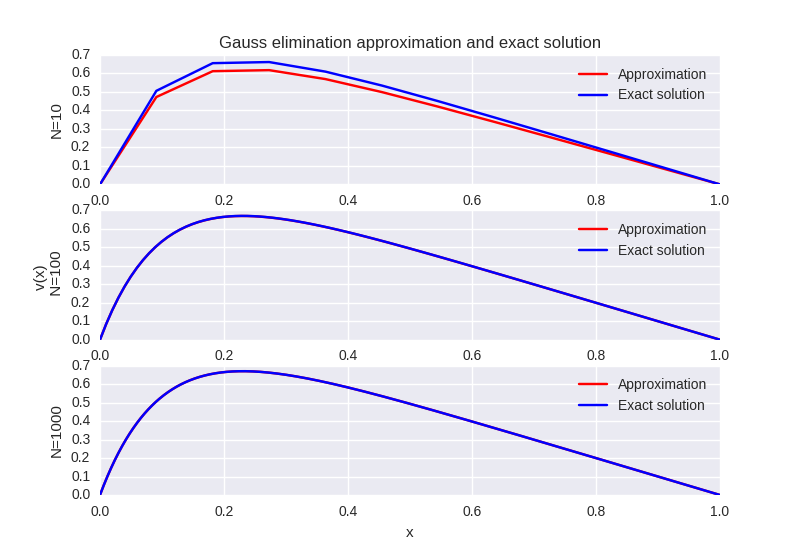
\includegraphics[scale=0.8]{Gaussian_comparison.png}
\caption{Plot of $u(x)$ and $v(x)$ for various N}
\end{figure}

\end{flushleft}

\subsection*{CPU times}

\begin{flushleft}
All methods were run $100$ times for $N=10, 10^2, 10^3$, and the computed average CPU time can be found in Figure $5$. Simulations were also run for $N=10 000$, but the LU-decomposition took too long to yield any results. In contrast to the Gaussian og specialized methods used here, which are customized for tridiagonal matrices and leave the $0$-elements untouched, the LU-decomposition of the matrix performs permutations on \textit{all} matrix elements. This makes for a much higher number of flops and longer CPU time, as we can see from the results. For larger $N$ the LU-decomposition becomes increasingly slower.
\end{flushleft}

\begin{figure}[ht]\label{CPU times N=1,2,3}
\centering
\begin{tabular}{|c|c|c|c|}
\hline
Step length  & Gaussian & Specialized & LU-decomposition \\
$\log_{10}(h)$ & & & \\
\hline
$-1$ & $1.65e-06$ & $1.5e-06$& $1.072e-05$\\
$-2$ & $1.183e-05$ & $1.06e-05$ & $0.0008079$ \\
$-3$ & $0.00011527$ & $0.00010371$ & $0.64698$\\
\hline
\end{tabular}
\caption{CPU times of simulations}
\end{figure}

\subsection*{Errors}

\begin{flushleft}
The relative error of an approximation is calculated using the formula \cite{hjorth2011computational}

\begin{equation}
\epsilon_i = \log_{10} \Big( \Big| \frac{v_i-u_i}{u_i} \Big| \Big) 
\end{equation}

Where $v_i$ is the approximated value and $u_i$ is the exact value at $x_i$. All methods were run for $N=10, 10^3, 10^5, 10^7$, and the maximum error was returned. Results are found in Figure $6$. It's apparent that the error is indeed of the order of $h^2$, as mentioned in the Methods section. For $N=10^7$ the error in the Gaussian method was very small and virtually zero for the specialized method. For $N=10^4$ and larger, the simulation using LU-decomposition yielded an error message, complaining about the lack of space.
\end{flushleft}

\begin{figure}[ht]\label{Relative errors}
\centering
\begin{tabular}{|r|c|c|c|}
\hline
$\log_{10}(h)$ & Gaussian & Specialized & LU-decomposition \\
\hline
$-1$ & $-1.1797$ & $-1.1797$ & $-1.1797$ \\
$-3$ & $-5.08005$ & $-5.08005$ & $-5.08005$\\
$-5$ & $-9.0049$ & $-9.08055$ & Not enough memory\\
$-7$ & $-13.007$ & $-\infty$ & Not enough memory\\
\hline
\end{tabular}
\caption{Relative errors}
\end{figure}

\section*{Discussion}

\begin{flushleft}
For a small number of iterations $N$ the Gaussian method for tridiagonal matrices, our specialized method and the LU-decomposition yield similar errors and CPU times. As the number of iterations increases, however, the LU-decomposition becomes very uneffective. In fact, for $N>4$ it is useless.
\end{flushleft}


\nocite{*}

\bibliography{referanser}{}
\bibliographystyle{plain}

\section*{Appendix}

\begin{flushleft}
\textbf{Error of three point method}

Calculate the mathematical error (?)
\end{flushleft}




\end{document}